\documentclass[12pt]{article}
\usepackage[english]{babel}
\usepackage{graphicx, amsmath, amsfonts, amsthm, mathtools, listings, color, caption, rotating, subfigure, fullpage, textcomp, enumerate, float, listings, MnSymbol, wasysym}

\lstset{
	language=Python,
	keywordstyle=\bfseries\ttfamily\color[rgb]{0,0,1},
	identifierstyle=\ttfamily,
	commentstyle=\color[rgb]{0.133,0.545,0.133},
	stringstyle=\ttfamily\color[rgb]{0.627,0.126,0.941},
	showstringspaces=false,
	basicstyle=\tiny,
	numberstyle=\scriptsize,
	numbers=left,
	stepnumber=1,
	numbersep=10pt,
	tabsize=2,
	breaklines=true,
	breakatwhitespace=false,
	aboveskip={1.5\baselineskip},
  columns=fixed,
  upquote=true,
  extendedchars=true,
}

\begin{document}
\begin{center}
Cats and Dogs Final Report\\
June 9, 2014, STA298\\
Christopher Aden, Chuan Qi, Nick Ulle\\
\end{center}

\section{Introduction}
The Cats and Dogs problem intially comes from Kaggle.com's Dogs vs. Cats competition. The purpose of the comeptition was to guage how far along image recognition has come in detecting dogs versus cats (a task proposed as an alternative to reCAPTCHA to verify that a user is a human and not a computer). Using support vector machines, (Golle, 2008) was able to achieve 82.7\% classification rate, training on color and texture features from an image. Our training set involves 20,000 images: pictures of dogs and cats with file names indicating whether they were a dog or cat. Our test set consists of 5,000 images with no tags. The objective is to determine whether an image in the test set is a cat or a dog, with a high degree of accuracy, based on a model created using the training data.

The purpose of this project is to demonstrate that deep learning is a more effective method for classifying images than the previous standard established in Golle's paper. 

\section{Approaches--The Successful and The Failed}
We tried four fundamentally different approaches to classifying the images.

While we ultimately decided to use the OverFeat software for classification,
we originally considered implementing our own algorithm as well.
The intention was that we could find something with better interpretability,
albeit with some loss of accuracy.
One approach we found for this, based on a paper by Coates and Ng,
was to use spherical k-means clustering for feature extraction.
In particular, each image in the training set is divided into 16 by 16 patches
of pixels, and spherical k-means clustering is applied to produce a dictionary of features.
To classify a test image, 
first each patch of the image is mapped to an entry in the feature dictionary.
Many different mappings are possible;
typically there is some tradeoff between efficiency and accuracy.
The number of occurences of each feature can then be counted---although this
is not the only approach---and provided to an apprporiately-trained linear
classifier.

This k-means-based approach to the problem had the potential to be easily
interpretable: our hope was that many patches in the feature dictionary would
have a clear correspondence to either cats or dogs.
Moreover, the original paper was flexible to the needs of the reader.
A wide array of possibilities for tuning and adjusting were presented,
which would have given us many avenues for improving accuracy.

Spherical k-means clustering is sufficiently exotic that we could find no
pre-existing libraries implementing it, so we wrote our own implementation.
A major concern was how well the algorithm would scale to our very large
training set, and we made preliminary investigations into moving our
Python code to Cython.
Due to the astounding success of OverFeat on the data set, and the fact that
many of our group members dropped out or were doing this for fun rather than
credit, this was as far as we got with implementing the k-means clustering
strategy.

Nevertheless, this project was a learning experience.
The spherical version of the k-means clustering algorithm was unfamiliar to
all of us, as were the damped k-means updates advocated in the paper.
Additionally, we learned that it's important to set clear project goals early
on; our group was somewhat directionless until halfway through the quarter.






\subsection{K-means}
Use spherical K-means on scaled and ZCA-whitened chunks (e.g. 16x16) of the training images, in order to build up a dictionary of K features. Images can then be mapped to a vector of length K by representing each chunk with its closest entry in the dictionary, and summing over the keys for all chunks. Classify based on the chunks. (Classification Rate: \%)

\subsection{Pixel-Based Classifiers}
A very simple approach to classification is to work on the pixel level. Using the \verb+Image+ library in Python, we can turn each image into three matrices, each one with number of rows equal to the number of pixels wide the image is, and columns equal to the image's pixel height. The three matrices correspond to the intensity of red, blue, and green in the $(i,j)$ pixel. We then flatten each image into a width x height x 3 array of RGB pixel intensities. 

Doing this for all images in the training data, we then stack them into a matrix, scaling to make them all have the same width and height. The resolution chosen was 500 x 350, which was somewhat arbitrary. It was the mean resolution of ten arbitrarily-chosen images. Without the images being the same resolution, we would not have been able to put them all in a matrix.

This is now a very high dimensional classification, where we are attempting to predict a binary response (dog or cat) using the pixel intensities from the $500 \cdot 350 \cdot 3 = 525,000$ pixel dimensions. To reduce the ill-fitting nature of this classification, we apply principal components analysis to the pixel intensities. The hope is that the first few principal components of the dogs looks different from the first few principal components of the cats, and that we can use some discriminant to split them apart. The following plot shows the first two principal axes using this strategy.

\begin{figure}[H] \center
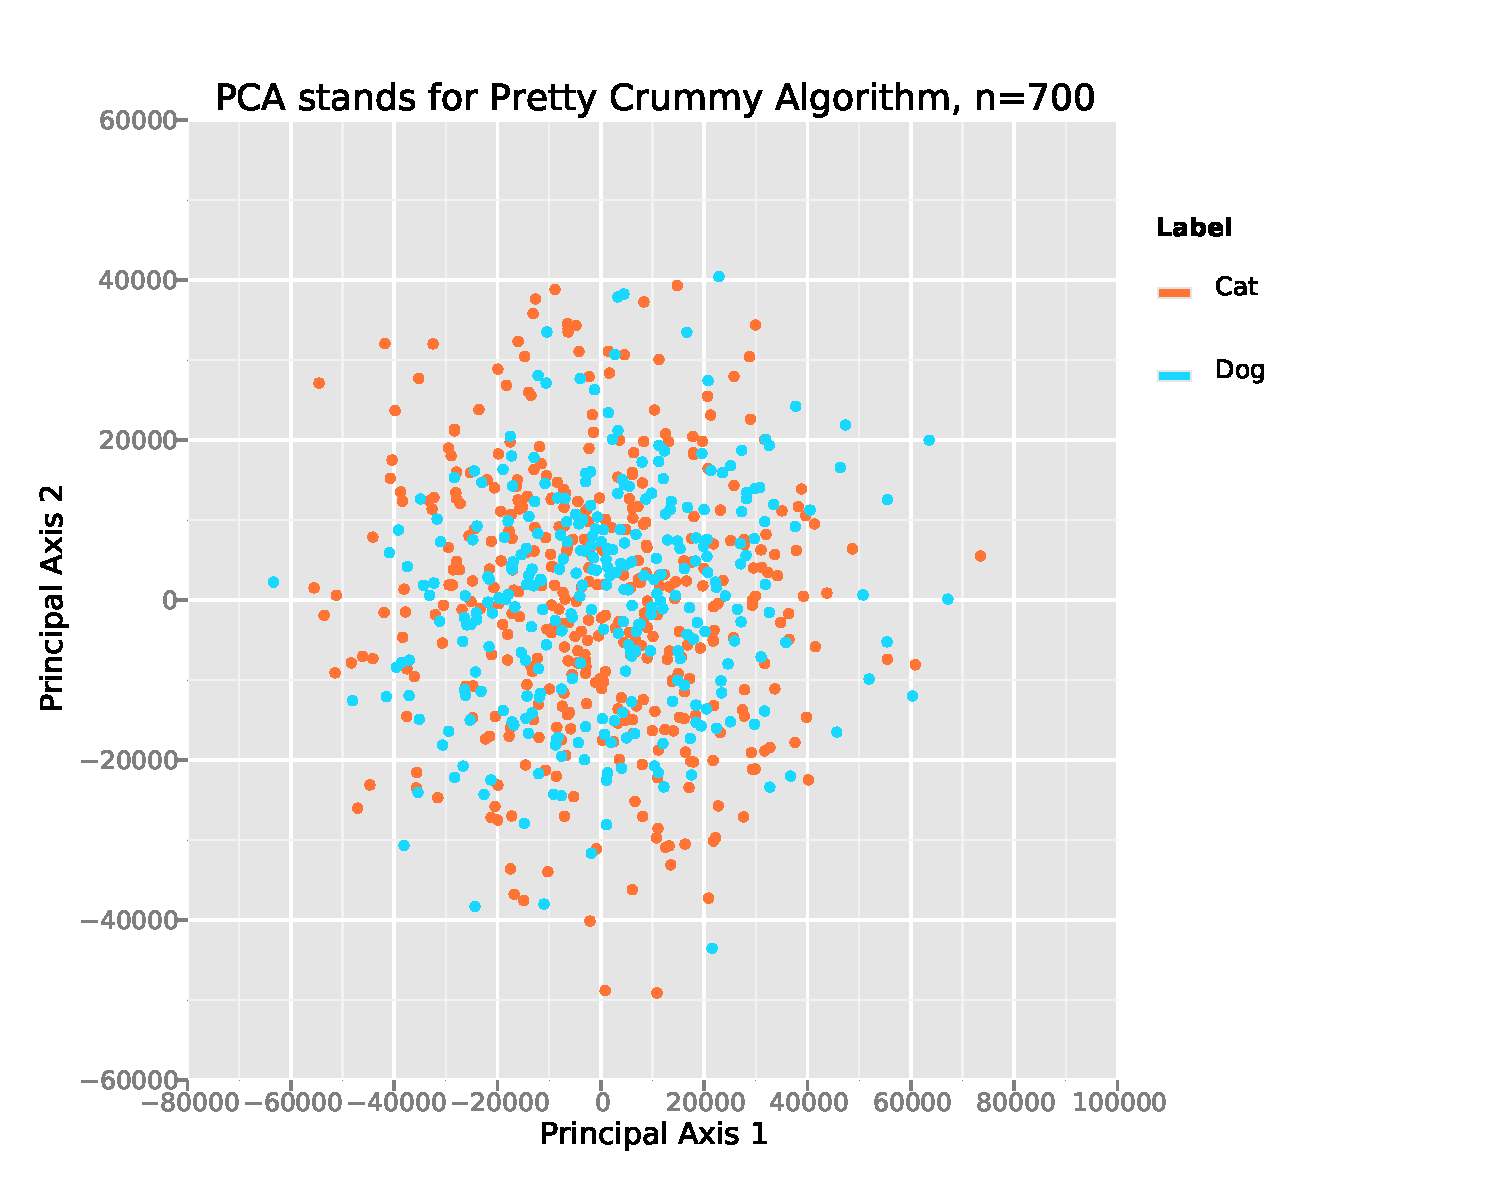
\includegraphics[scale=.50]{PCA_plot.pdf} 
\end{figure}

There is little to no difference between the dog and cat pixel values. This makes sense--we do not distinguish dogs from cats based on just color, and even that is difficult, because this method is not location-independent. A dog in the upper left will produce a completely different loading from a picture with the same dog in the bottom right. With a linear discriminant rule, this approach yields a classification rate less than 55\%. 

Attempting to use support vector machines instead on the principal loadings would allow for a non-linear discrimination rule. This solves very few of our problems, as is clear in its 57\% classification rate.

\subsection{Overfeat Feature Label Classifier}
It is clear that a pixel-only approach is not the best idea. There are too many features that operate on a scale bigger than the pixel level. From a biological perspective, we tend to evaluate dogs and cats on the shape of the ears, bushiness of tails, and the eyes. It would be smart if we had a method for picking out important features that were most indicative of ``cat-ness'' or ``dog-ness''. The OverFeat program and algorithm does exactly this. OverFeat implements a convolutional neural network, which attempts to find important features in an image. The neural network's feature selection is trained on the ImageNet database, a collection of 14.2 million images, each one tagged with relevant classes. This is generally a very time-intensive procedure, but OverFeat pre-trains the convolutional neural net, and classifying on an image takes less than ten seconds, since the CNN is written is C++ and compiled against an optimized BLAS.

The Overfeat program will, by default, output ImageNet categories. This classifier takes the ImageNet corpus for dog and cat words, and deterministically classifies an image as Dog or Cat, based on whether the most common feature word is a dog or cat word. If an image contains neither dog nor cat words, the image is randomly placed in Dog or Cat with equal probability. This method is very naive, and doesn't use any further machine learning techniques to classify, but still manages to drastically outperform pixel-based methods. On the training set, this method manages to correctly predict 88.7\% of the images. This demonstrates, more than anything, the power of the convolutional neural network in classifying images, as the classifier itself is extremely primitive.

\subsection{Overfeat Layer Classifiers}
In this approach, we extract the neural net layers from the Overfeat feature selection algorithm, pre-trained on ImageNet. This produces a large three-dimensional matrix of features. We apply the method of max-pooling, where we take the node with the largest activation, which involves taking the maximum over all columns, then the maximum over the depth of the matrix. The purpose is to reduce the feature space into something more manageable to avoid overfitting. This produces a 4096 x 1 vector from each image. The hard work complete, we try two classifiers to get the final labels.
\begin{description}
\item[SVM:] We use the labels and 4096-vectors to build a support vector machine with a variety of kernels on a subset of the data. Linear, cubic, and radial basis were used as kernels. Cross-validation on the training data gives us an estimate of which kernels will perform the best on the testing set. The extra complexity of the RBF proves useful, and it scores a slightly better classification rate. Cross-validated, our classification rate is 97.5\%, with linear and cubic kernels coming up a few percent behind.

\item[Neural Net:] We build a back-propagated neural network with 4096-length input layer and a 1D output layer. We play around with the number of hidden neurons and train until suitable number of iterations passes and our in-sample and out-of-sample error rates seem to converge. We use the trained neural net to predict testing observations for a classification rate of 96.9\%.
\end{description}

\section{Results}
%Using the CNN-SVM approach (since it scored the highest classification rate)

\section{Future Work}

\section{Most Important Things Learned}

\section{Appendix}
\subsection{References}
\begin{description}
\item[] Philippe Golle. 2008. Machine learning attacks against the Asirra CAPTCHA. In Proceedings of the 15th ACM conference on Computer and communications security (CCS '08). ACM, New York, NY, USA, 535-542. DOI=10.1145/1455770.1455838 http://doi.acm.org/10.1145/1455770.1455838
\item[] 
\end{description}

\subsection{Python Source Code}
%\lstinputlisting{"helper_functions.R"}
 
\end{document} 
